\documentclass[aspectratio=169, 10pt]{beamer}

% Theme & Typography
\usetheme{Madrid}
\usecolortheme{beaver}
\setbeamertemplate{navigation symbols}{}
\setbeamertemplate{headline}{}

\usepackage[utf8]{inputenc}
\usepackage{booktabs}
\usepackage{graphicx}
\usepackage{hyperref}
\usepackage{amsmath}
\usepackage{xcolor}

% Custom Editorial Palette
\definecolor{primaryDark}{RGB}{12, 10, 9}
\definecolor{accentAmber}{RGB}{180, 83, 9}
\definecolor{accentGreen}{RGB}{21, 128, 61}
\definecolor{accentBlue}{RGB}{3, 105, 161}

\setbeamercolor{title}{fg=white, bg=primaryDark}
\setbeamercolor{frametitle}{fg=white, bg=primaryDark}
\setbeamercolor{structure}{fg=primaryDark}

\title[GCC Atlas India]{\textbf{GCC Atlas India: Strategic Product Deck}}
\subtitle{A Neutral, Sourced Reference for Global Capability Centres}
\author[Product Intern Review]{Rajnish}
\institute[Flexiple]{Role: Product Intern Assignment \\ \medskip \href{https://givemehat.github.io/gcc-atlas-india/}{\textcolor{accentAmber}{\textbf{Live Application: https://givemehat.github.io/gcc-atlas-india/}}} \\ \href{https://github.com/givemehat/gcc-atlas-india}{\textcolor{accentBlue}{GitHub Repository: github.com/givemehat/gcc-atlas-india}}}
\date{October 2026}

\begin{document}

% SLIDE 1: TITLE SLIDE
\begin{frame}
  \titlepage
\end{frame}

% SLIDE 2: ECOSYSTEM FOUNDATION
\begin{frame}{Market Scale: Ground Truth vs Projections}
  \begin{columns}
    \begin{column}{0.48\textwidth}
      \begin{block}{Verified National Baseline (Nasscom-Zinnov FY26)}
        \begin{itemize}
          \item \textbf{2,117 GCC Corporate Parents}
          \item \textbf{3,728 Operating Units} nationwide
          \item \textbf{2.36 Million Professionals} in tech \& leadership
          \item \textbf{$\sim$\$98.4B Annual Value} exported to parent HQs
        \end{itemize}
      \end{block}
    \end{column}
    \begin{column}{0.48\textwidth}
      \begin{block}{Commercial Real Estate View (JLL 2026)}
        \begin{itemize}
          \item \textbf{200+ New Units Projected} over 24 months
          \item \textbf{Leasing Density:} Bengaluru \& Hyderabad lead absorption
          \item \textbf{Unit vs Parent Divergence:} Commercial lease deeds count branches separately from corporate parents
        \end{itemize}
      \end{block}
    \end{column}
  \end{columns}
\end{frame}

% SLIDE 3: THE PROBLEM
\begin{frame}{The Problem}
  \begin{columns}
    \begin{column}{0.54\textwidth}
      \begin{itemize}
        \item \textbf{The Players:} Global entrants, commercial landlords, BOT advisors, legal/tax firms, recruiters, EOR platforms, and state IT agencies.
        \item \textbf{The Epistemic Disparity:} Reports contradict on Bengaluru:
          \begin{itemize}
            \item \textit{Vestian (Jul 2025):} 487 GCCs (standalone parent leases)
            \item \textit{JLL India (Jan 2026):} 900+ units (physical business units)
            \item \textit{Flexiple (Feb 2026):} $\sim$870 GCCs (entity-level hubs)
          \end{itemize}
        \item \textbf{Who is Hurt (Hypotheses to Validate):}
          \begin{itemize}
            \item \textit{Entrant CXO:} Prolonged feasibility cycles and risk of broker-driven corridor misallocation.
            \item \textit{Service Providers:} Quality delivery-first operators lose bids to marketing-heavy incumbents.
          \end{itemize}
        \item \textbf{What They Do Today:} Rely on informal referrals and unverified PDF consultant summaries.
      \end{itemize}
    \end{column}
    \begin{column}{0.44\textwidth}
      \begin{figure}[htbp]
        \centering
        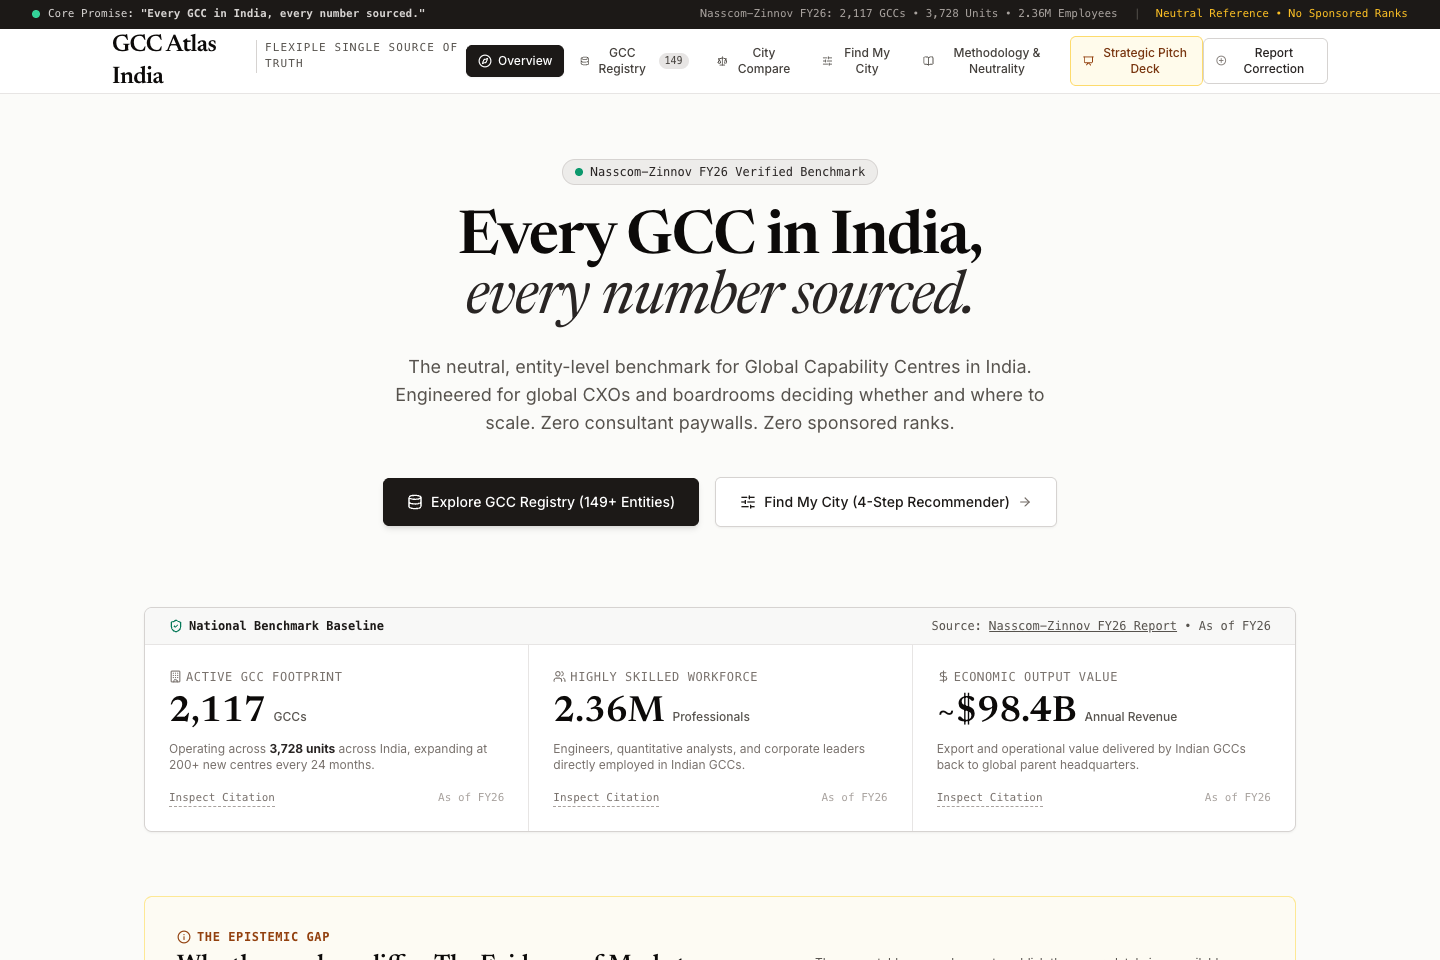
\includegraphics[width=\textwidth]{public/screenshots/01_overview_home.png}
        \caption{\footnotesize Epistemic Disparity Panel on Home Page}
      \end{figure}
    \end{column}
  \end{columns}
\end{frame}

% SLIDE 4: THE OPPORTUNITIES
\begin{frame}{The Opportunities}
  \begin{columns}
    \begin{column}{0.5\textwidth}
      \textbf{Which Matter Most \& Why (Prioritization):}
      \begin{enumerate}
        \item \textbf{Entity Sourced Registry (Priority \#1):}
          \begin{itemize}
            \item \textit{Why:} Trust is the prerequisite. Verifiable corporate filing links establish epistemic authority.
          \end{itemize}
        \item \textbf{Deterministic Location Recommender (Priority \#2):}
          \begin{itemize}
            \item \textit{Why:} Captures uncorrupted entrant buyer intent (sector, team size, priority).
          \end{itemize}
        \item \textbf{Multi-City Benchmark Matrix (Priority \#3):}
          \begin{itemize}
            \item \textit{Why:} Delivers instant board-ready numbers on rents, talent cost arbitrage, and state policy gazettes.
          \end{itemize}
      \end{enumerate}
    \end{column}
    \begin{column}{0.48\textwidth}
      \begin{block}{Full Ecosystem Landscape}
        \begin{itemize}
          \item \textbf{A.} Entity Sourced Registry (Live)
          \item \textbf{B.} Deterministic Recommender (Live)
          \item \textbf{C.} City Comparator Matrix (Live)
          \item \textbf{D.} Regulatory Ingestion Pipeline (Future exploration: MCA Form MGT-7 crawler)
          \item \textbf{E.} Talent Mobility Radar (Future exploration: Leadership departures)
          \item \textbf{F.} Audited Provider Directory
          \item \textbf{G.} Vetted RFP Marketplace
        \end{itemize}
      \end{block}
    \end{column}
  \end{columns}
\end{frame}

% SLIDE 5: THE SOLUTION (REGISTRY & COMPARATOR)
\begin{frame}{The Solution: Audited Registry \& Comparator Matrix}
  \begin{columns}
    \begin{column}{0.54\textwidth}
      \begin{block}{149 Audited GCC Records (Data Honesty)}
        \begin{itemize}
          \item \textbf{AUDIT.md Results:} 126 Confirmed Unchanged (84.6\%), 20 Corrected to primary portals (13.4\%), 3 Nulled for honesty (2.0\%), 0 Fabricated.
          \item \textbf{Strict Null Policy:} Unstated fields (e.g. Stripe headcount/year) strictly nulled as \textit{"Not available yet"}.
          \item \textbf{Confidence Tiers:} 131 Verified, 16 Reported, 2 Estimated.
        \end{itemize}
      \end{block}
      \begin{block}{6-City Head-to-Head Comparator}
        \begin{itemize}
          \item Benchmarks Bengaluru, Hyderabad, Pune, Chennai, Delhi NCR, Mumbai.
          \item Grade A blended rents \& min-max corridor spreads.
          \item Tech salary bands + discount vs Bengaluru baseline.
          \item Official State IT Policies (Karnataka, Telangana, TN).
        \end{itemize}
      \end{block}
    \end{column}
    \begin{column}{0.44\textwidth}
      \begin{figure}[htbp]
        \centering
        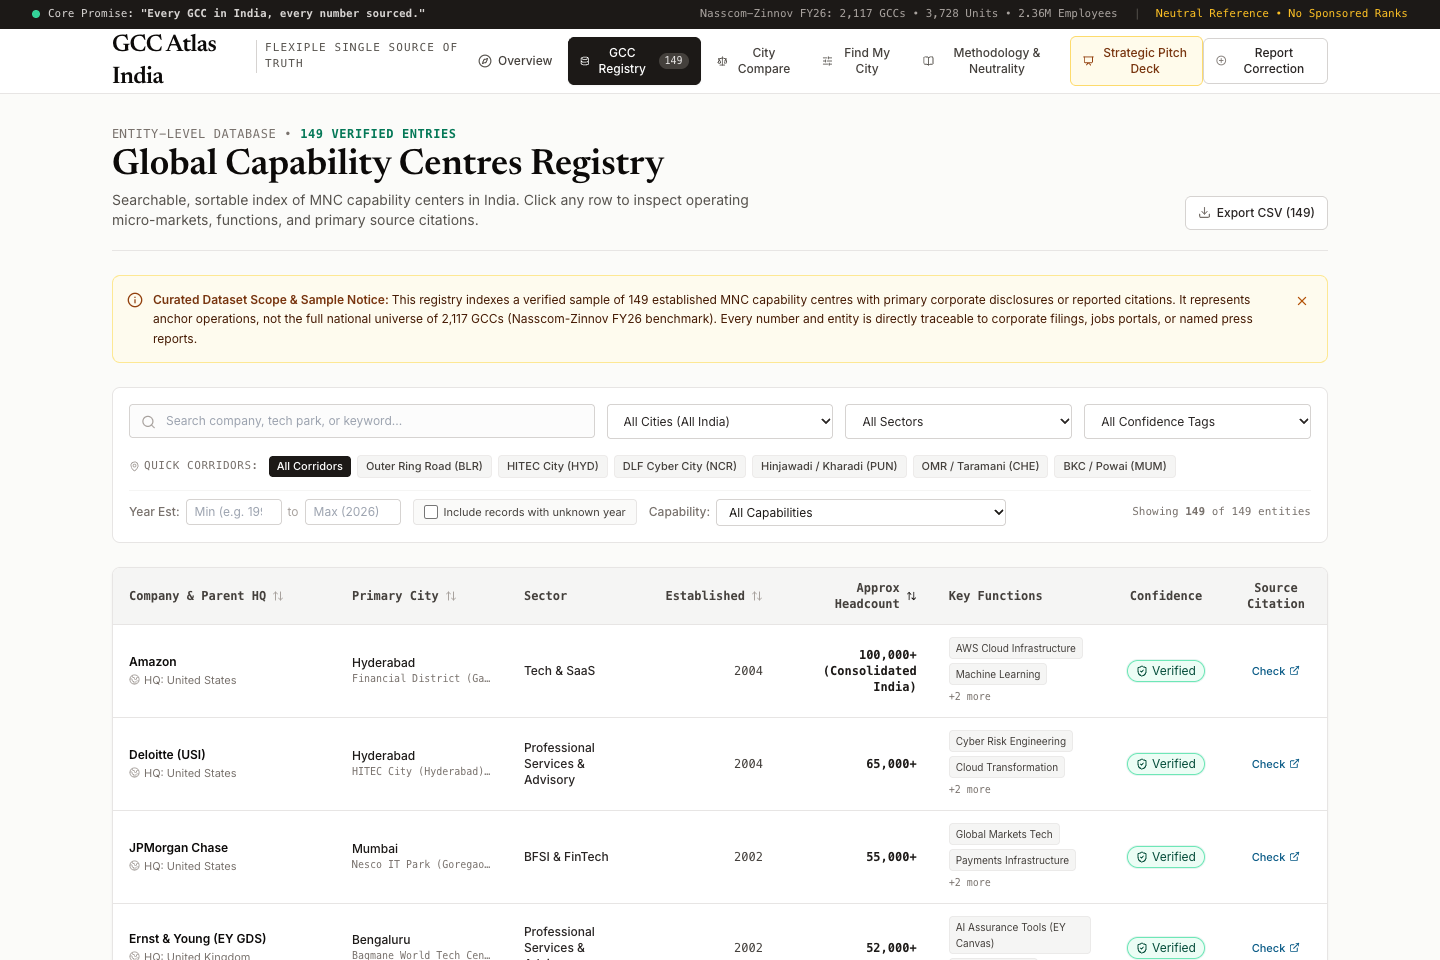
\includegraphics[width=\textwidth]{public/screenshots/02_entity_registry.png}
        \caption{\footnotesize Live Entity Registry with Corridor Filters}
      \end{figure}
      \vspace{-0.2cm}
      \begin{figure}[htbp]
        \centering
        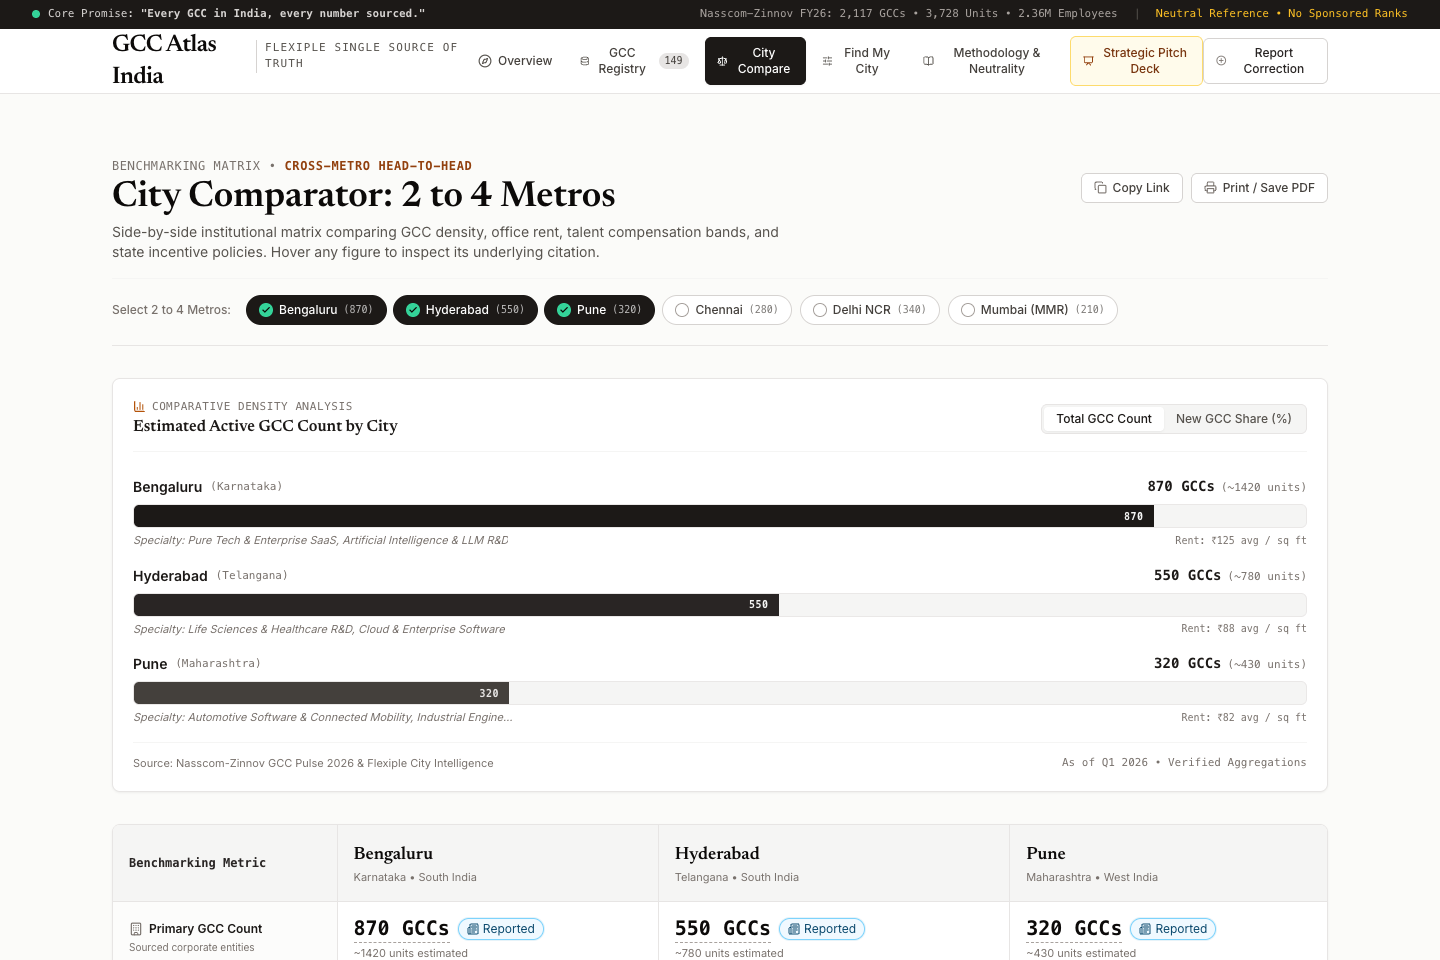
\includegraphics[width=\textwidth]{public/screenshots/03_city_compare.png}
        \caption{\footnotesize 6-City Matrix Comparator \& SVG Density Chart}
      \end{figure}
    \end{column}
  \end{columns}
\end{frame}

% SLIDE 6: THE SOLUTION (LOCATION RECOMMENDER)
\begin{frame}{The Solution: Deterministic Location Recommender}
  \begin{columns}
    \begin{column}{0.52\textwidth}
      \begin{itemize}
        \item \textbf{Target Persona First:} Global CXO / VP of Engineering setting up a 100--1,000 engineer hub.
        \item \textbf{4 Strategic Criteria:} Sector, 3-Year Headcount ($<$100, 100--500, 500--2000, 2000+), Primary Mandate, Decisive Priority (40\% Weight).
        \item \textbf{Transparent Scoring Formula:}
          $$\text{Score} = (\text{Priority} \times 4.0) + \text{Sector} (25) + \text{Function} (20) + \text{Scale} (15) + \text{Base} (10)$$
        \item \textbf{Ranked Top 3 Output:} Exact match \%, plain-language rank justifications, real peer GCC anchors, and honest caveats (e.g. ORR traffic, BKC rent premiums).
      \end{itemize}
    \end{column}
    \begin{column}{0.46\textwidth}
      \begin{figure}[htbp]
        \centering
        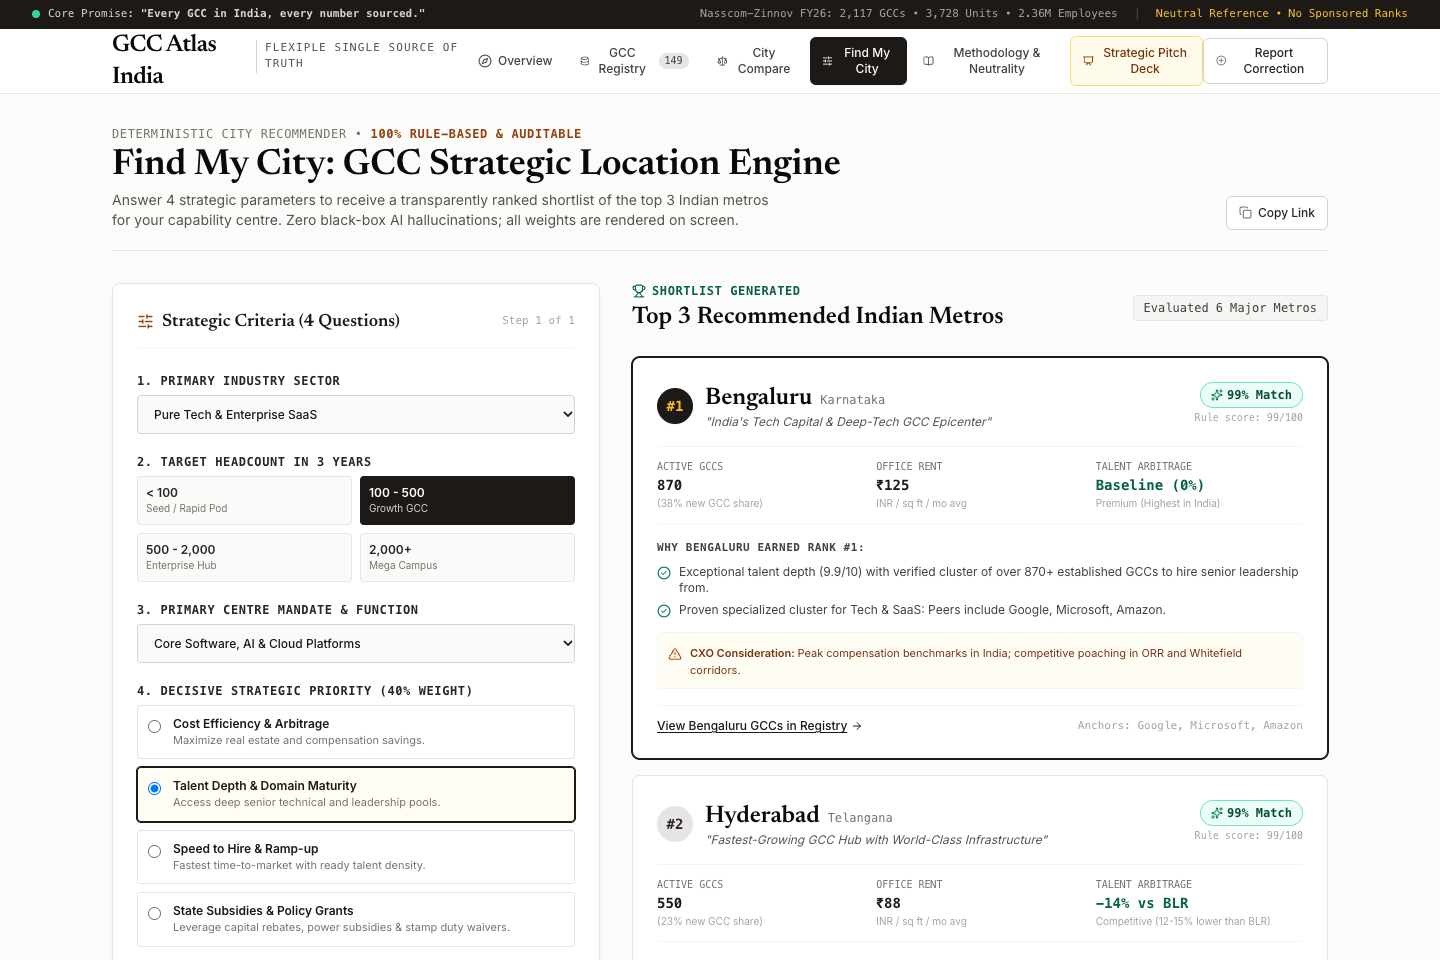
\includegraphics[width=\textwidth]{public/screenshots/04_find_my_city.png}
        \caption{\footnotesize Find My City: Auditable scoring rule \& breakdown table}
      \end{figure}
    \end{column}
  \end{columns}
\end{frame}

% SLIDE 7: THE POSITIONING
\begin{frame}{The Positioning: A Neutral, Sourced Reference}
  \begin{columns}
    \begin{column}{0.54\textwidth}
      \textbf{Brand Wedge:} \textit{"A Neutral, Sourced Reference \& Decision Guide."}
      \begin{itemize}
        \item \textbf{The Neutrality Rule:} Nobody can pay to alter a ranking, boost a score, or remove an honest caveat.
        \item \textbf{Entrant-Free Model:} Global companies access 100\% of the data without paywalls.
      \end{itemize}
      \smallskip
      \begin{block}{Why Each Stakeholder Switches to GCC Atlas}
        \begin{itemize}
          \item \textbf{Global CXO:} Zero cost, primary filing citations, 5-minute decision clarity instead of vague consultant decks.
          \item \textbf{Setup Advisors \& BOTs:} High-intent inbound RFP leads from CXOs who have finalized their shortlist.
          \item \textbf{Commercial Developers:} Real-time corridor-level demand intelligence (ORR, HITEC, Kharadi, BKC).
          \item \textbf{State Governments:} Sourced showcase of gazetted policy incentives delivered to active decision-makers.
        \end{itemize}
      \end{block}
    \end{column}
    \begin{column}{0.44\textwidth}
      \begin{figure}[htbp]
        \centering
        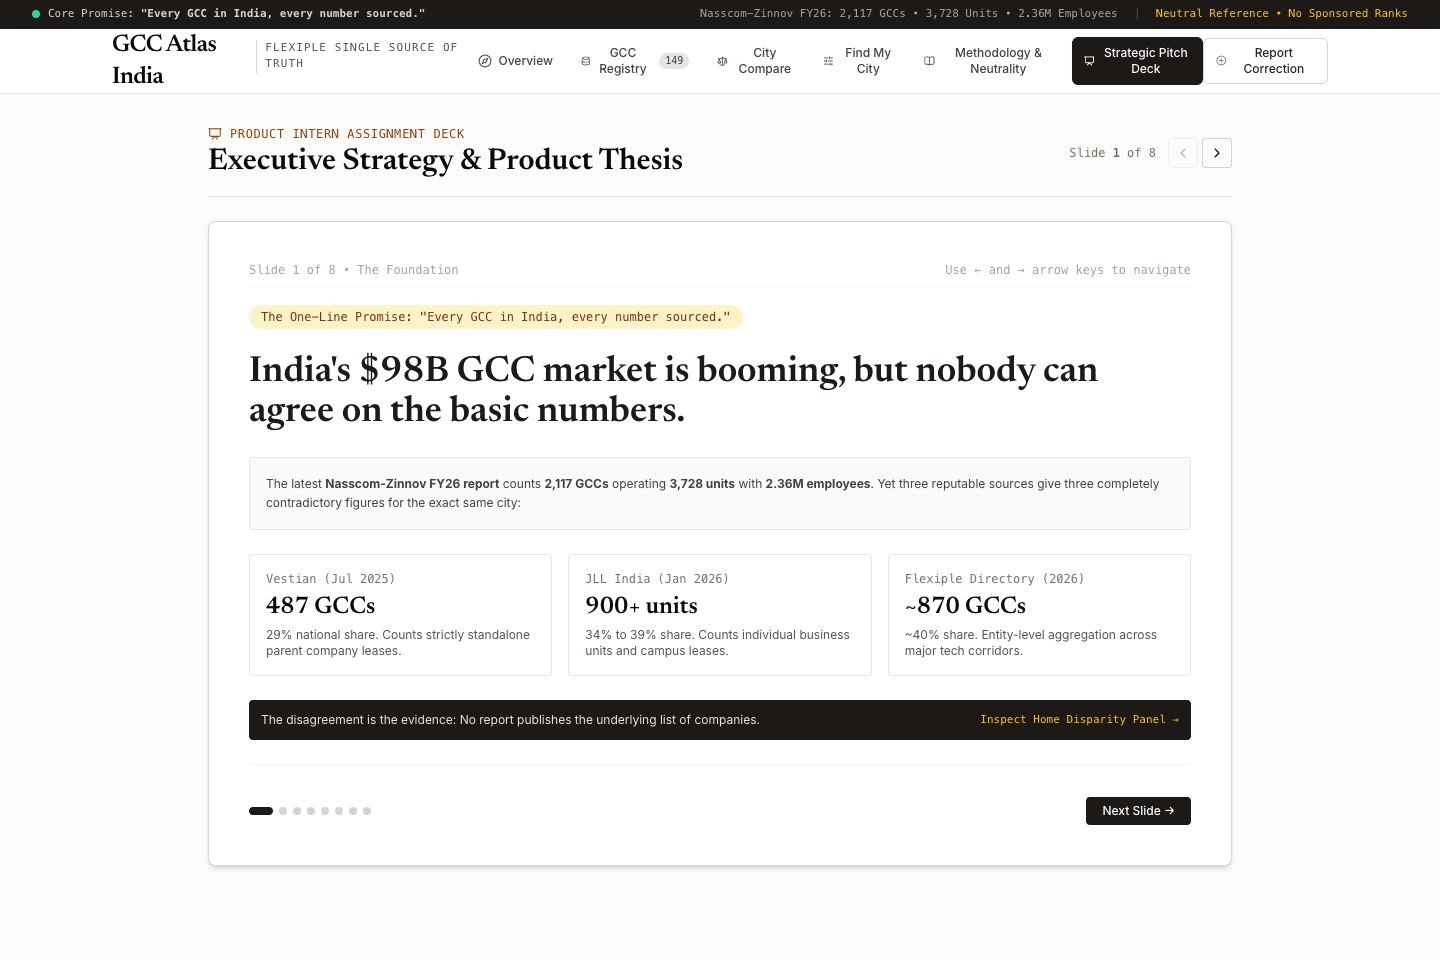
\includegraphics[width=\textwidth]{public/screenshots/05_pitch_deck.png}
        \caption{\footnotesize In-app Strategic Deck Viewer \& Governance Rules}
      \end{figure}
    \end{column}
  \end{columns}
\end{frame}

\end{document}
